\documentclass[main.tex]{subfiles}

\begin{document}

\begin{center}
{\Large \bf{Modeling the uncertainties of solar-system ephemerides\\
for robust gravitational-wave searches with pulsar timing arrays}}\\
\end{center}

\begin{multicols}{2}
Vallisneri, Taylor, Simon, et al. 2020\\
arXiv:

Corresponding author:\\
% Michele Vallisneri\\
\href{mailto:michele.vallisneri@jpl.nasa.gov}{michele.vallisneri@jpl.nasa.gov}

\end{multicols}

\vspace{-3ex}

\rule{\textwidth}{1pt}

\setlength\intextsep{0pt} %no vertical space
\setlength{\columnsep}{10pt} %minimal horizontal space

%\begin{wrapfigure}{R}{0pt}
%\centering
%\vspace{-25pt}
%\includegraphics[trim={0 10ex 0 20ex},clip,width=0.9\textwidth]{gravitational_wave_spectrum.png}
%\includegraphics[trim={15ex 0 10ex 0},clip,width=0.55\textwidth]{f2.pdf}
%\caption*{{\it Modeling of the arrival-time delays with the standard NANOGrav methodology. We also show the trajectory of the pulsar on the sky with the delay amplitudes overlaid.}}
%\vspace{11pt}
%\end{wrapfigure}

The abundance and precision of pulsar-timing-array datasets is now so great that our sensitivity to gravitational waves is limited by the accuracy to which we can position Earth around the barycenter of the solar system. A 100-km error in our estimate of the orbit of Jupiter creates a 100-m apparent barycenter wobble, which appears as a 30-ns slowly evolving delay in pulse times of arrival---very much like gravitational waves. Accordingly, adopting different solar-system ephemerides among the few most recent leads to different posterior probability distributions for the gravitational-wave amplitude (see dashed lines in Fig.\ 1).

To make NANOGrav's search for stochastic backgrounds in the 11-yr dataset robust to these errors, we developed \textsc{BayesEphem}, a physical model of ephemeris uncertainties that focuses on the degrees of freedom that most affect our search---indeed, Jupiter's orbital elements. After marginalizing over \textsc{BayesEphem} parameters, the gravitational-wave posteriors look the same no matter which ephemeris we adopt (see solid lines in Fig.\ 1). Modeling ephemeris errors does reduce our sensitivity to gravitational waves, but this limitation will disappear as pulsar timing datasets become longer, and as better estimates of Jupiter's orbit become available, notably thanks to the measurements of the Juno mission.

While our analysis does not update current ephemerides significantly, it provides entirely independent uncertainty estimates. See Fig.\ 2 for the NANOGrav bounds on Jupiter's orbit, compared to the intrinsic error estimates of JPL ephemeris DE436. In the future we will consider the sector of ephemeris corrections that do not affect gravitational-wave results, but that may benefit from pulsar-timing-array constraints, thus producing pulsar-timing-enhanced ephemerides useful beyond gravitational-wave detection.

Visit {\it nanograv.org} to learn more about NANOGrav.

\vspace{12pt}
\begin{figure}[h]
\centering
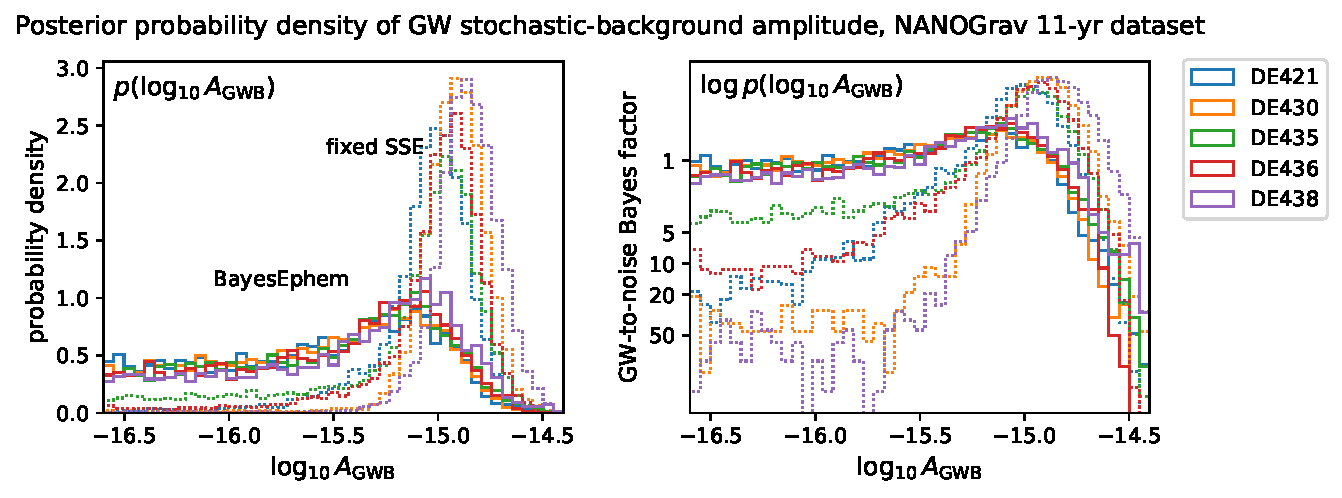
\includegraphics[width=0.8\textwidth]{GWposterior.pdf}
\caption{Posterior probability of gravitational-wave stochastic-background amplitude at $f=1\,\mathrm{yr}^{-1}$ under different JPL ephemerides (DE421--DE438), with (solid) and without (dashed) \textsc{BayesEphem}.}
\end{figure}

\vspace{12pt}

\begin{figure}[h]
\centering
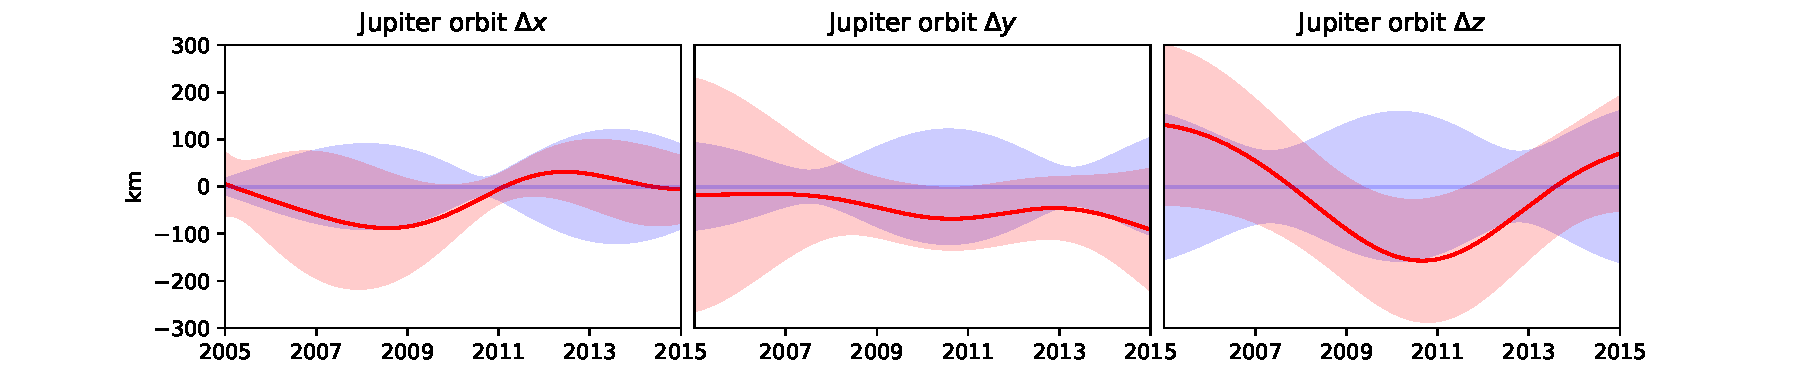
\includegraphics[width=0.8\textwidth]{orbit-corrections.pdf}
\caption{\textsc{BayesEphem} corrections to Jupiter's orbit in JPL ephemeris DE436 (red: mean and 2-$\sigma$ contours) vs.\ DE436 estimated uncertainty (blue: 2-$\sigma$ contours).}
\end{figure}

\end{document}





